\documentclass[12pt]{report}
\usepackage[utf8]{inputenc}
\usepackage[russian]{babel}
\linespread{1.5}
%\usepackage[14pt]{extsizes}
\usepackage{listings}
\usepackage{float}
\usepackage{graphicx}
\usepackage[left=2cm,right=2cm,
    top=2cm,bottom=2cm,bindingoffset=0cm]{geometry}
\usepackage{amsmath,amsfonts,amssymb,amsthm,mathtools} 

% Для листинга кода:
\lstset{ %
language=swift,                
basicstyle=\small\sffamily, % размер и начертание шрифта для подсветки кода
numbers=left,               % где поставить нумерацию строк (слева\справа)
numberstyle=\tiny,           % размер шрифта для номеров строк
stepnumber=1,                   % размер шага между двумя номерами строк
numbersep=5pt,                % как далеко отстоят номера строк от подсвечиваемого кода
showspaces=false,            % показывать или нет пробелы специальными отступами
showstringspaces=false,      % показывать или нет пробелы в строках
showtabs=false,             % показывать или нет табуляцию в строках
frame=single,              % рисовать рамку вокруг кода
tabsize=2,                 % размер табуляции по умолчанию равен 2 пробелам
captionpos=t,              % позиция заголовка вверху [t] или внизу [b] 
breaklines=true,           % автоматически переносить строки (да\нет)
breakatwhitespace=false, % переносить строки только если есть пробел
escapeinside={\#*}{*)}   % если нужно добавить комментарии в коде
}

% Для измененных титулов глав:
%\usepackage{titlesec, blindtext, color} % подключаем нужные пакеты
%\definecolor{gray75}{gray}{0.75} % определяем цвет
%\newcommand{\hsp}{\hspace{20pt}} % длина линии в 20pt
% titleformat определяет стиль
%\titleformat{\chapter}[hang]{\Huge\bfseries}{\thechapter\hsp\textcolor{gray75}{|}\hsp}{0pt}{\Huge\bfseries}

\usepackage{titlesec}
\titleformat{\chapter}[block]
  {\normalfont\huge\bfseries}{\thechapter.}{1em}{\Huge}
\titlespacing*{\chapter}{0pt}{-19pt}{0pt}


% plot
\usepackage{pgfplots}
\usepackage{filecontents}
\usetikzlibrary{datavisualization}
\usetikzlibrary{datavisualization.formats.functions}
\newenvironment{comment}{}{}
\begin{comment}
\begin{filecontents}{LevR.dat}
1 5928
2 16865
3 62333
4 372661
5 1909255
6 9065189
7 45325069
\end{filecontents}

\begin{filecontents}{LevT.dat}
1 3724258
2 7224736
3 12123365
4 16940041
5 23402008
6 32328258
7 30166031
\end{filecontents}

\begin{filecontents}{DamLevR.dat}
1 7456
2 21845
3 105445
4 407763
5 1966658
6 11002094
7 51219656
\end{filecontents}

\begin{filecontents}{DamLevT.dat}
1 4367560
2 8286833
3 12852145
4 18585284
5 24103230
6 27935583
7 30567571
\end{filecontents}
\end{comment}

\begin{document}
%\def\chaptername{} % убирает "Глава"
\begin{titlepage}

	\fontsize{12pt}{12pt}\selectfont
	\noindent \begin{minipage}{0.15\textwidth}
		
\includegraphics[width=\linewidth]{b_logo.jpg}
	\end{minipage}
	\noindent\begin{minipage}{0.9\textwidth}\centering
		\textbf{Министерство науки и высшего образования Российской Федерации}\\
		\textbf{Федеральное государственное бюджетное образовательное учреждение высшего образования}\\
		\textbf{«Московский государственный технический университет имени Н.Э.~Баумана}\\
		\textbf{(национальный исследовательский университет)»}\\
		\textbf{(МГТУ им. Н.Э.~Баумана)}
	\end{minipage}
	
	\noindent\rule{18cm}{3pt}
	\newline\newline
	\noindent ФАКУЛЬТЕТ $\underline{\textbf{«Информатика и системы управления»}}$ \newline\newline
	\noindent КАФЕДРА $\underline{\textbf{«Программное обеспечение ЭВМ и информационные технологии»}}$\newline\newline\newline\newline
	
	\begin{center}
		\Large\textbf{Отчет по лабораторной работе №1 по курсу <<Анализ алгоритмов>>}
	\end{center}
	\newline\newline 
	\newline
	
	\noindent\textbf{Тема} $\underline{\textbf{Расстояние Левенштейна~~~~~~~~~~~~~~~~~~~~~~~~~~~}}$\newline\newline
	\noindent\textbf{Студент} $\underline{\textbf{Челядинов И.Д.~~~~~~~~~~~~~~~~~~~~~~~~~~~~~~~~~}}$\newline\newline
	\noindent\textbf{Группа} $\underline{\textbf{ИУ7-53Б~~~~~~~~~~~~~~~~~~~~~~~~~~~~~~~~~~~~~~~~~~~~}}$\newline\newline
	\noindent\textbf{Оценка (баллы)} $\underline{\textbf{~~~~~~~~~~~~~~~~~~~~~~~~~~~~~~~~~~~~~~~~~~}}$\newline\newline
	\noindent\textbf{Преподаватели} $\underline{\textbf{Волкова Л.Л., Строганов Ю.В.}}$\newline
	
	\begin{center}
		\vfill
		Москва~---~\the\year
		~г.
	\end{center}
 \restoregeometry
\end{titlepage}


\tableofcontents

\newpage
\chapter*{Введение}
\addcontentsline{toc}{chapter}{Введение}
\textbfb Расстояние Левенштейна - минимальное количество операций вставки одного символа, удаления одного символа и замены одного символа на другой, необходимых для превращения одной строки в другую.

Расстояние Левенштейна применяется в теории информации и компьютерной лингвистике в следующих случаях:

\begin{itemize}
	\item исправления ошибок в слове(поисковая строка браузера);
	\item сравнения текстовых файлов утилитой diff;
	\item в биоинформатике для сравнения генов, хромосом и белков.
\end{itemize}

Целью данной лабораторной работы является изучение метода динамического программирования на материале алгоритмов
Левенштейна и Дамерау-Левенштейна. 

Задачами данной лабораторной являются:
\begin{itemize}
  	\item изучение алгоритмов Левенштейна и Дамерау-Левенштейна нахождения расстояния между строками;
	\item применение метода динамического программирования для матричной реализации указанных алгоритмов; 
	\item получение практических навыков реализации указанных алгоритмов: двух алгоритмов в матричной версии и двух алгоритмов в рекурсивной версии; 
	\item сравнительный анализ линейной и рекурсивной реализаций выбранного алгоритма определения расстояния между строками по затрачиваемым ресурсам (времени и памяти); 
	\item экспериментальное подтверждение различий во временнóй эффективности рекурсивной и
нерекурсивной реализаций выбранного алгоритма определения расстояния между строками при
помощи разработанного программного обеспечения на материале замеров процессорного времени
выполнения реализации на варьирующихся длинах строк; 
	\item описание и обоснование полученных результатов в отчете о выполненной лабораторной работе, выполненного как расчётно-пояснительная записка к работе. 
\end{itemize}


\chapter{Аналитическая часть}
Задача по нахождению расстояния Левенштейна заключается в поиске минимального количества операций вставки/удаления/замены для превращения одной строки в другую.

При нахождении расстояния Дамерау — Левенштейна добавляется операция транспозиции (перестановки соседних символов).  
 
\textbfДействия обозначаются слдующим образом: 
\begin{enumerate}
  	\item D (англ. delete) — удалить;
	\item I (англ. insert) — вставить;
	\item R (replace) — заменить;
	\item M(match) - совпадение.
\end{enumerate}

Пусть $S_{1}$ и $S_{2}$ — две строки (длиной M и N соответственно) над некоторым алфавитом, тогда расстояние Левенштейна можно подсчитать по следующей рекуррентной формуле (1.1):

\begin{equation}
D(i,j) = \left\{ \begin{array}{ll}
 0, & \textrm{$i = 0, j = 0$}\\
 i, & \textrm{$j = 0, i > 0$}\\
 j, & \textrm{$i = 0, j > 0$}\\
min(\\
D(i,j-1)+1,\\
D(i-1, j) +1, &\textrm{$j>0, i>0$}\\
D(i-1, j-1) + m(S_{1}[i], S_{2}[j])\\
),
  \end{array} \right.
\end{equation}

где $m(a,b)$ равна нулю, если $a=b$ и единице в противном случае; $min\{\,a,b,c\}$ возвращает наименьший из аргументов.

Расстояние Дамерау-Левенштейна вычисляется по следующей рекуррентной формуле (1.2):

\begin{equation}	    
D(i, j) =  \left\{
	\begin{aligned}
		&0, && i = 0, j = 0\\
		    	&i, && i > 0, j = 0\\
		    	&j, && i = 0, j > 0\\		    	
		    	&min \left\{
				\begin{aligned}
					&D(i, j - 1) + 1,\\
		            &D(i - 1, j) + 1,\\
		            &D(i - 1, j - 1) + m(S_{1}[i], S_{2}[i]), \\
		            &D(i - 2, j - 2) + m(S_{1}[i], S_{2}[i]),\\
		        \end{aligned} \right.
		        && 
				\begin{aligned}
					&, \text{ если } i, j > 0 \\
		            & \text{ и } S_{1}[i] = S_{2}[j - 1] \\
		            & \text{ и } S_{1}[i - 1] =  S_{2}[j] \\
		        \end{aligned} \\ 
		        &min \left\{
		        \begin{aligned}
		            &D(i, j - 1) + 1,\\
		            &D(i - 1, j) + 1, \\
		            &D(i - 1, j - 1) + m(S_{1}[i], S_{2}[i]),\\
		        \end{aligned} \right.  &&, \text{иначе}
			\end{aligned} \right.
\end{equation}
\section*{Вывод}
	В данном разделе были рассмотрены алгоритмы нахождения расстояния Левенштейна и Дамерау-Левенштейна, который является модификаций первого, учитывающего возможность перестановки соседних символов. 




\chapter{Конструкторская часть}
\textbf{Требования к программе:}
\begin{enumerate}
	\item На вход подаются две строки.
	\item Буквы в верхнем регистре и в нижнем регистре считаются разными.
  	\item Две пустые строки - корректный ввод, программа не должна аварийно завершаться.
  	\item Для всех алгоритмов выводиться процессорное время исполнения.
  	\item Для всех алгоритмов кроме Левенштейна с рекурсивной реализацией должна выводиться матрица.
\end{enumerate}

\section{Схемы алгоритмов}
В данной части будут рассмотрены схемы следующих алгоритмов Левенштейна : рекурсивного алгоритма Левенштейна (рис. 2.1), рекурсивного алгоритма Левенштейна с матричной оптимизацией (рис. 2.2),  матричного алгоритма Левенштейна (рис. 2.3), матричного алгоритма Левенштейна (рис. 2.4).\cite{Levenshtein}
\newpage
\newpage
На рисунке 2.1 представлен алгоритм поиска расстояния Левенштейна рекурсивно
\begin{figure}[h]
    \centering
    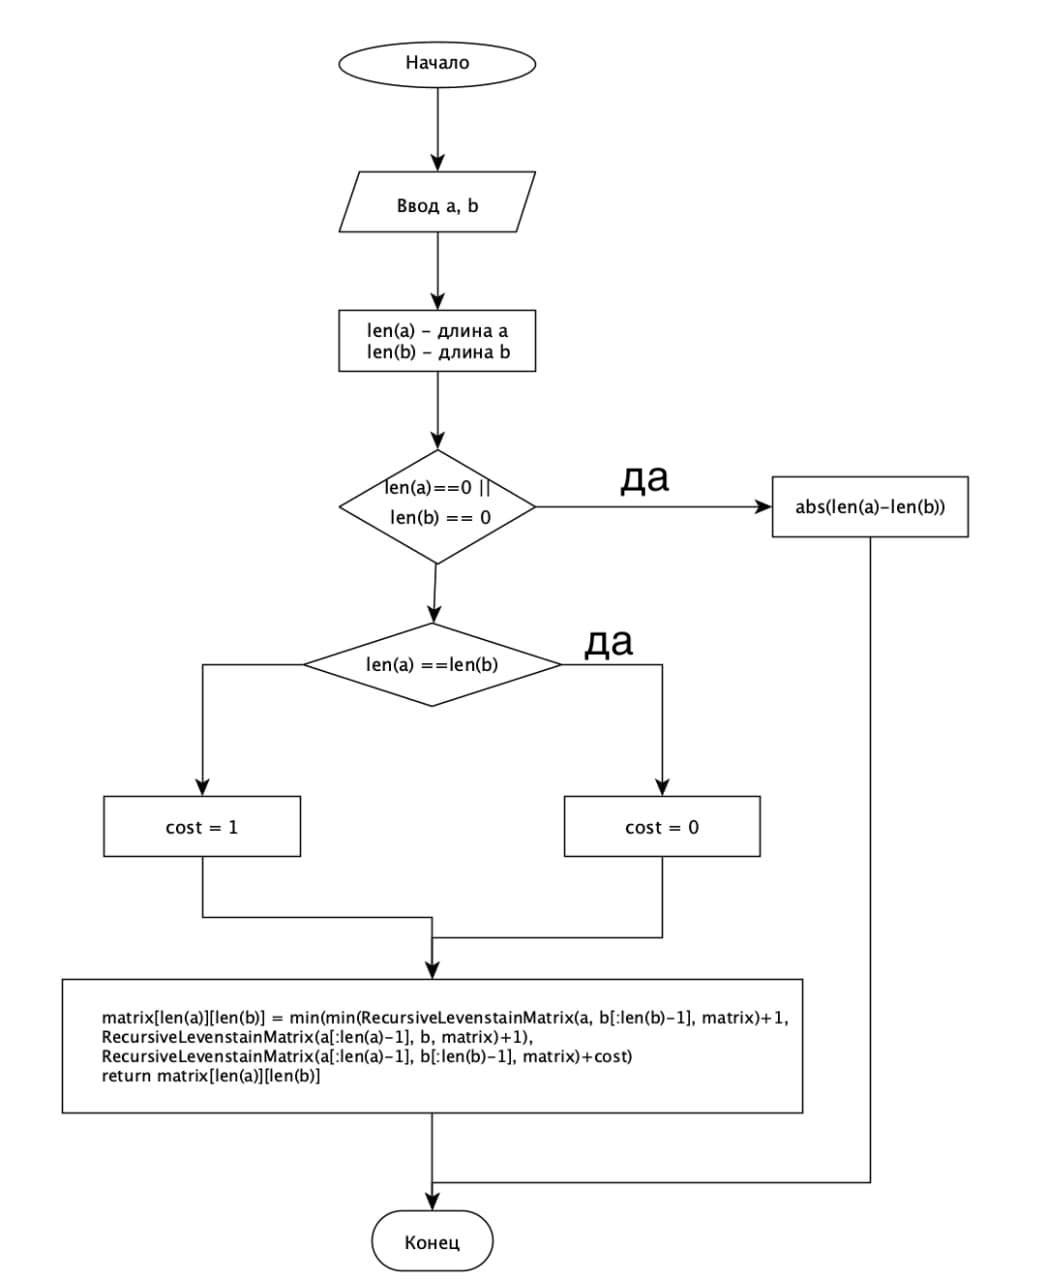
\includegraphics[width=0.70\linewidth]{rLev.jpg}
    \caption{Схема рекурсивного алгоритма нахождения расстояния Левенштейна}
    \label{fig:mpr}
\end{figure}

\newpage
\newpage
На рисунке 2.2 представлен алгоритм поиска расстояния Левенштейна рекурсивно с матричной оптимизацией
\begin{figure}[h]
    \centering
    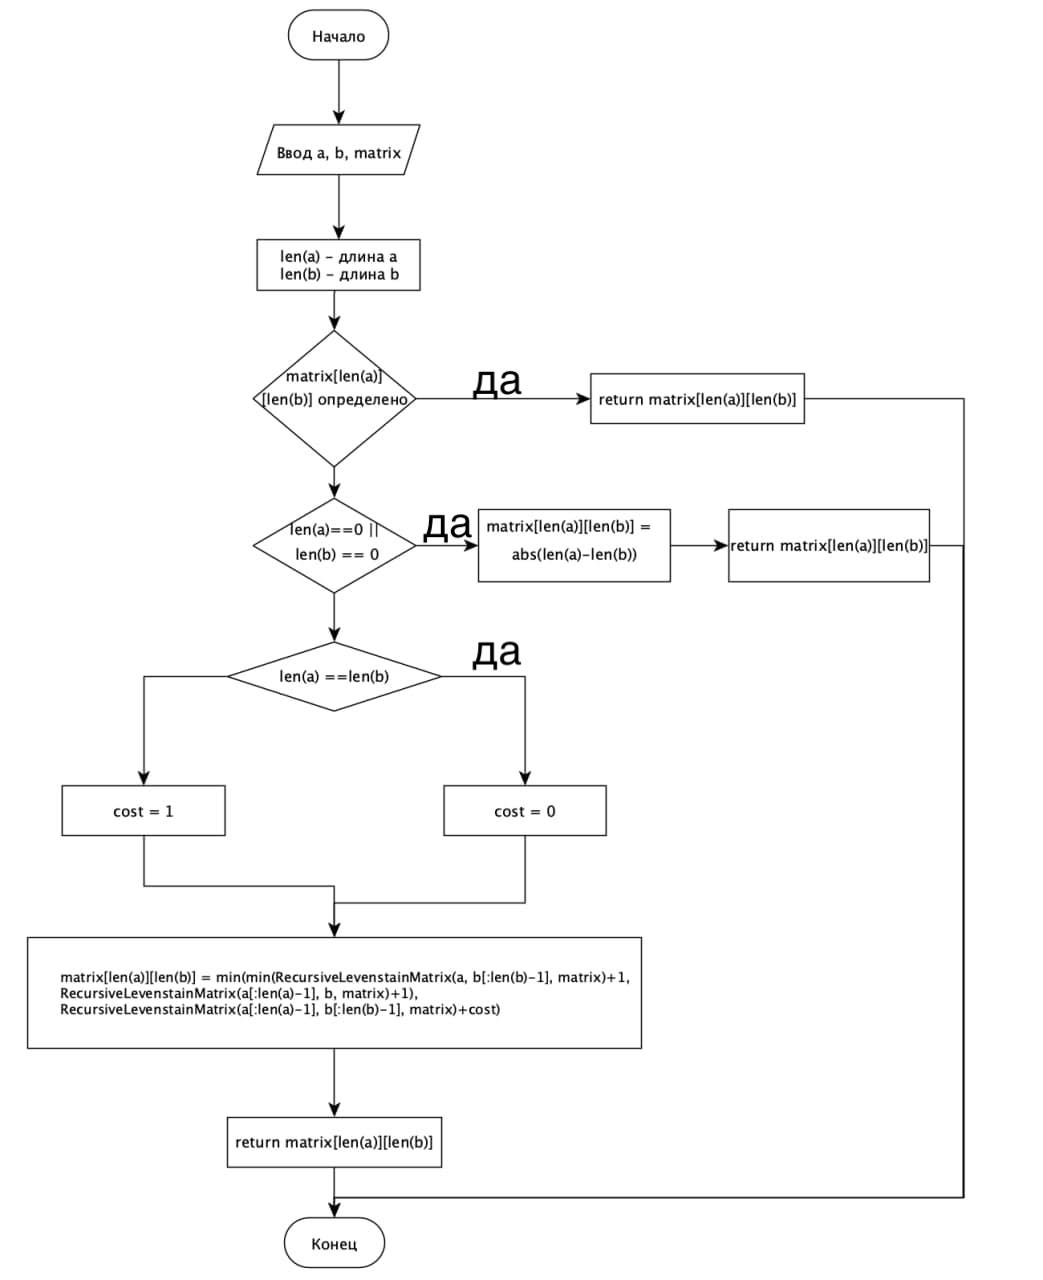
\includegraphics[width=0.70	\linewidth]{2.jpg}
    \caption{Схема рекурсивного алгоритма нахождения расстояния Левенштейна с матричной оптимизацией}
    \label{fig:mpr}
\end{figure}

\newpage
\newpage
На рисунках 2.3 - 2.4 представлен алгоритм поиска расстояния Левенштейна матрично
\begin{figure}[H]
    \centering
    \caption{}
    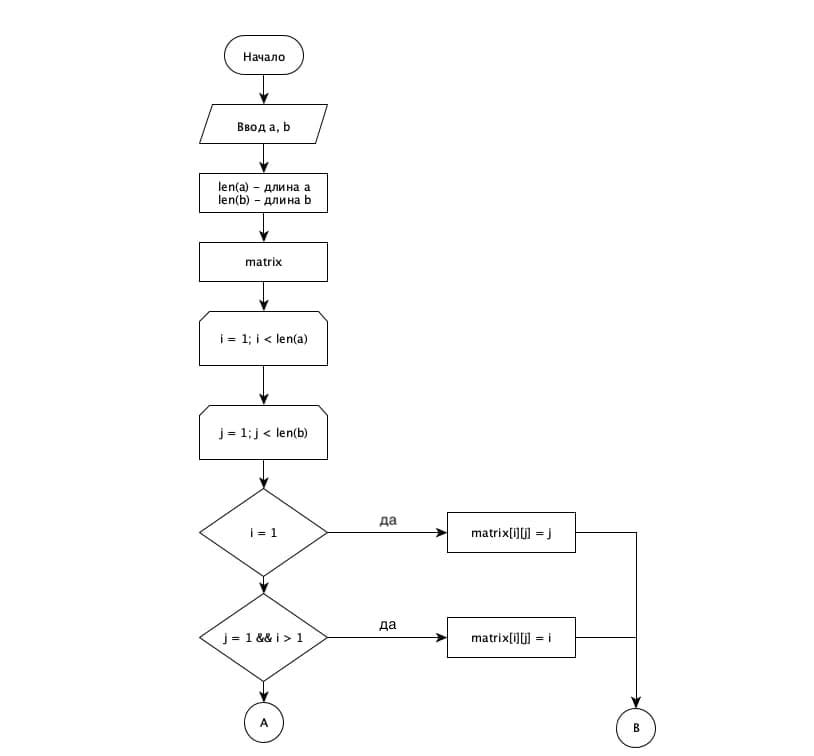
\includegraphics[width=0.80\linewidth]{3_1.jpeg}
    \label{fig:mpr}
\end{figure}

\begin{figure}[H]
    \centering
    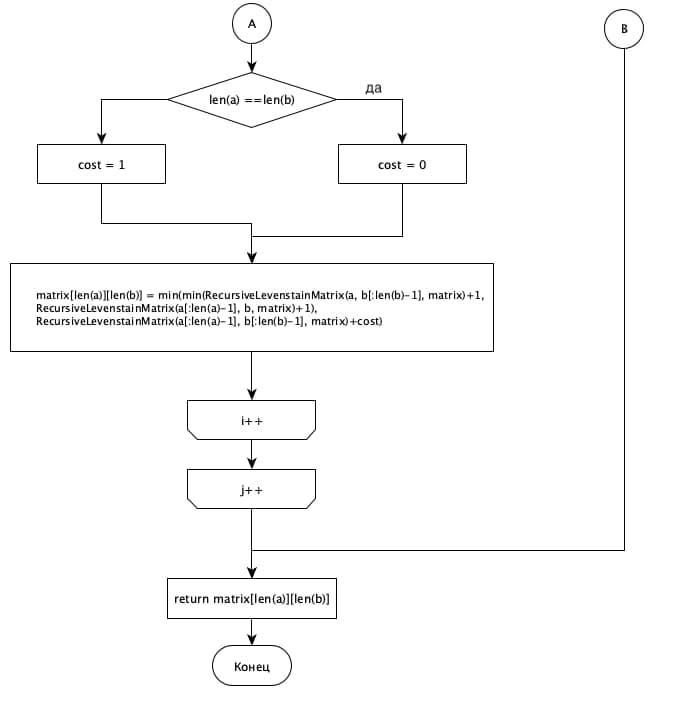
\includegraphics[width=1\linewidth]{3_2.jpg}
    \caption{Схема матричного алгоритма нахождения расстояния Левенштейна}
    \label{fig:mpr}
\end{figure}
На рисунках 2.5 - 2.6 представлен алгоритм поиска расстояния Дамерау-Левенштейна матрично
\begin{figure}[H]
    \centering
    \caption{}
    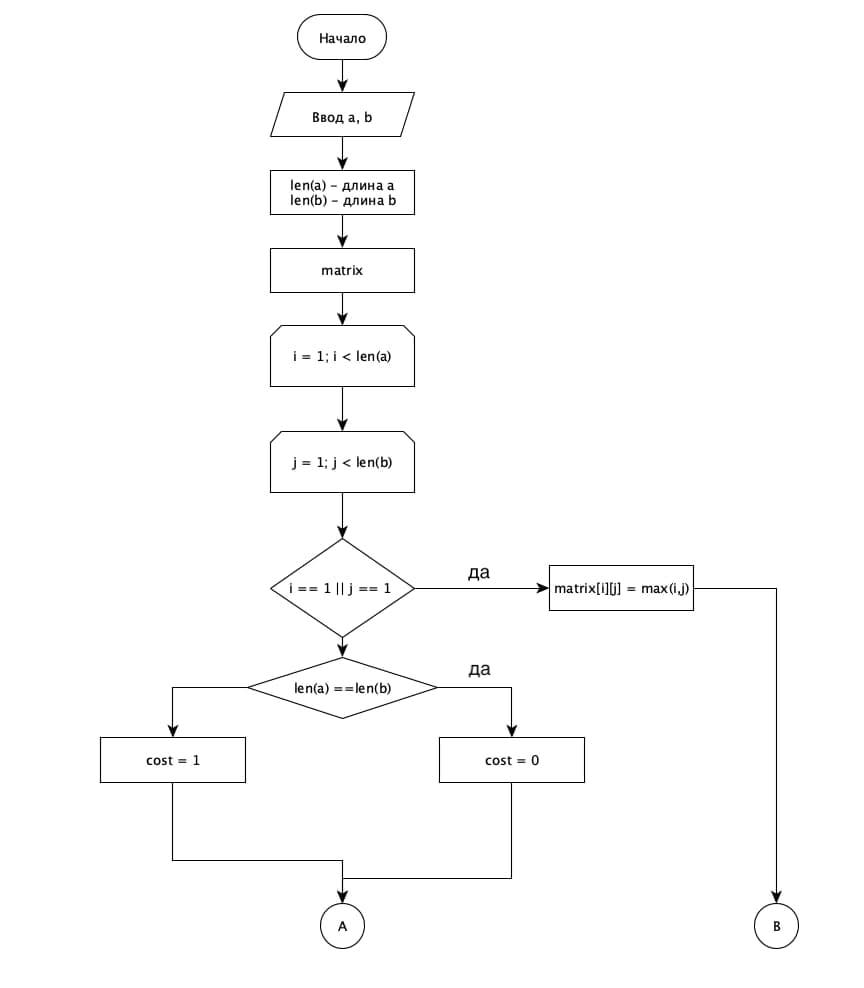
\includegraphics[width=0.80\linewidth]{4_1.jpg}
    \label{fig:mpr}
\end{figure}

\begin{figure}[H]
    \centering
    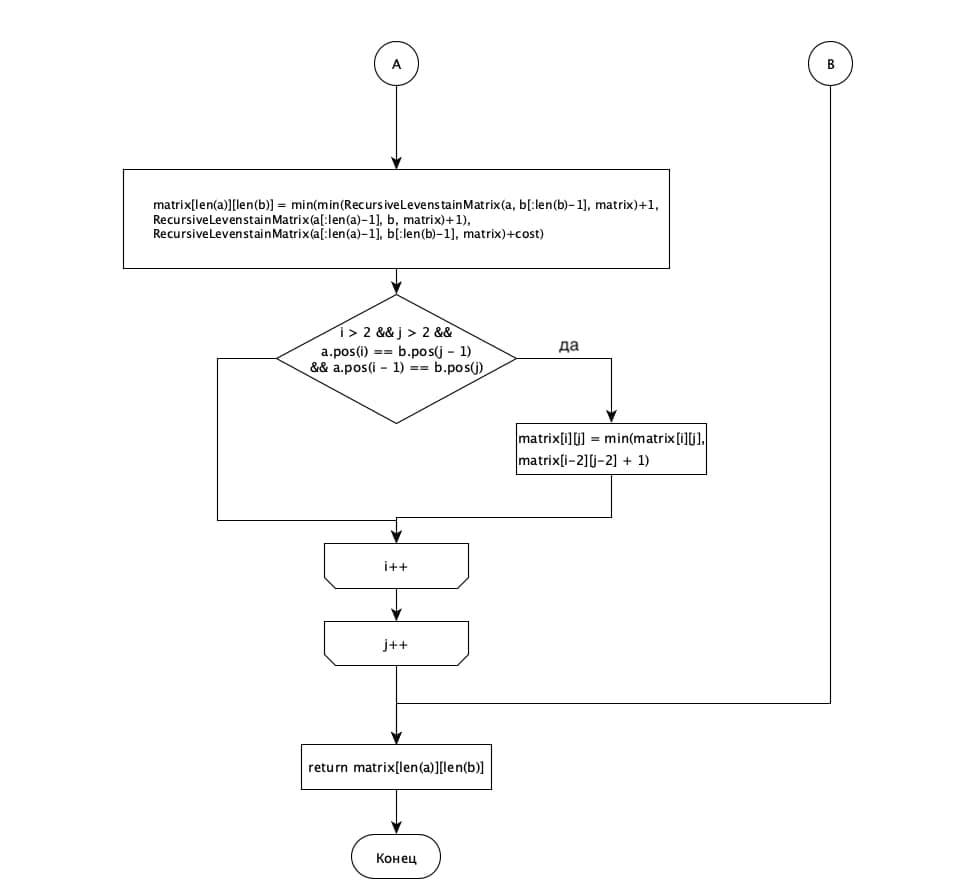
\includegraphics[width=0.8\linewidth]{4_2.jpg}
    \caption{Схема матричного алгоритма нахождения расстояния Дамерау-Левенштейна}
    \label{fig:mpr}
\end{figure}
\newpage



\section*{Вывод}
В данном разделе были рассмотрены требования к работе, а также схемы алгоритмов нахождения редакционного расстояния с помощью алгоритмов Левенштейна и Дамерау-Левенштейна.
\chapter{Технологическая часть}
\section{Выбор ЯП}
Для реализации программы был выбран язык программирования Golang в связи с потребностью практики разработки на нем. Среда разработки - Goland .\cite{golang} \cite{vscode}

\section{Реализация алгоритма}

В листинге 3.1 представлена функция нахождения расстояния Левенштейна рекурсивно
\begin{lstlisting}[label=some-code,caption=Функция нахождения расстояния Левенштейна рекурсивно]
func RecursiveLevenstain(a, b []rune) int {
	var cost int
	if len(a) == 0 || len(b) == 0 {
		return int(math.Abs(float64(len(a) - len(b))))
	}
	cost = 1
	if a[len(a)-1] == b[len(b)-1] {
		cost = 0
	}

	return min(min(RecursiveLevenstain(a, b[:len(b)-1])+1,
		RecursiveLevenstain(a[:len(a)-1], b)+1), RecursiveLevenstain(a[:len(a)-1], b[:len(b)-1])+cost)
}
\end{lstlisting}


В листинге 3.2 представлена функция нахождения расстояния Левенштейна рекурсивно с матрицей

\begin{lstlisting}[label=some-code,caption=Функция нахождения расстояния Левенштейна рекурсивно с матрицей]
func RecursiveLevenstainMatrix(a, b []rune, matrix [][]int) int {
	var cost int
	if len(a) == 0 || len(b) == 0 {
		matrix[len(a)][len(b)] = int(math.Abs(float64(len(a) - len(b))))
	}
	if matrix[len(a)][len(b)] != -1 {
		return matrix[len(a)][len(b)]
	}
	cost = 1
	if a[len(a)-1] == b[len(b)-1] {
		cost = 0
	}

	matrix[len(a)][len(b)] = min(min(RecursiveLevenstainMatrix(a, b[:len(b)-1], matrix)+1,
		RecursiveLevenstainMatrix(a[:len(a)-1], b, matrix)+1),
		RecursiveLevenstainMatrix(a[:len(a)-1], b[:len(b)-1], matrix)+cost)
	return matrix[len(a)][len(b)]
}
\end{lstlisting}


В листинге 3.3 представлена функция нахождения расстояния Левенштейна матрично

\begin{lstlisting}[label=some-code,caption=Функция нахождения расстояния Левенштейна матрично]
func MatrixLevenstain(a, b []rune, matrix [][]int) int {
	var cost int
	for i := 0; i < len(a)+1; i++ {
		for j := 0; j < len(b)+1; j++ {
			if i == 0 {
				matrix[i][j] = j
			} else if j == 0 && i > 0 {
				matrix[i][j] = i
			} else {
				cost = 1
				if a[i-1] == b[j-1] {
					cost = 0
				}
				matrix[i][j] = min(min(matrix[i][j-1]+1,
					matrix[i-1][j]+1),
					matrix[i-1][j-1]+cost)
			}
		}
	}
	return matrix[len(a)][len(b)]
}
\end{lstlisting}


В листинге 3.4 представлена функция нахождения расстояния Дамерау-Левенштейна матрично.

\begin{lstlisting}[label=some-code,caption=Функция нахождения расстояния Дамерау-Левенштейна матрично]
func DamerauLevenstainMatrix(a, b []rune, matrix [][]int) int {
	var cost int
	for i := 0; i < len(a)+1; i++ {
		for j := 0; j < len(b)+1; j++ {
			if i == 0 || j == 0 {
				matrix[i][j] = max(i, j)
			} else {
				cost = 1
				if a[i-1] == b[j-1] {
					cost = 0
				}
				matrix[i][j] = min(min(matrix[i][j-1]+1,
					matrix[i-1][j]+1),
					matrix[i-1][j-1]+cost)
				if j > 1 && i > 1 &&
					a[i-1] == b[j-2] &&
					a[i-2] == b[j-1] {
					matrix[i][j] = min(min(matrix[i][j], matrix[i-2][j-2]+1),matrix[i][j])
				}
			}
		}
	}
	return matrix[len(a)][len(b)]
}
\end{lstlisting}

В листинге 3.5 представлен код функций поиска минимума и максимума из двух чисел.
\begin{lstlisting}[label=some-code, caption=Функции поиска минимума и максимума]
func min(a, b int)int {
	if a > b{
		return b
	}
	return a
}
func max(a, b int) int{
	if a < b{
		return b
	}
	return a
}
\end{lstlisting}

\chapter{Исследовательская часть}

\section{Сравнительный анализ на основе замеров времени работы алгоритмов}

Был проведен замер времени работы каждого из алгоритмов. Замер производился на ноутбуке Macbook pro 13 на базе процессоре Intel core i5, который обладает  1.4 GHz тактовой частоты, а также 8 гигабайтами оперативной памяти.\cite{computer}\cite{intel} Для произведения замера времени использовалась система тестирования Benchmark языка Golang.
Данная система тестирования позволяет измерить скорость работы алгоритма с минимальной погрешностью. \newline
На рисунке 4 представлена зависимость времени исполнения функций от длины слова.\newline
\begin{tikzpicture}[H]
    \begin{axis}[
    	axis lines = left,
    	xlabel={Длина  (в символах)},
    	ylabel={Время (в наносекундах)},
    	xmin=1, xmax=10,
    	ymin=1, ymax=500,
    	legend pos=north west,
    	ymajorgrids=true
        ]
        \addplot[color=red] table[x index=0, y index=1] {LevR.dat}; 
        \addplot[color=orange] table[x index=0, y index=1] {LevRecM.dat};
        \addplot[color=blue, mark=square] table[x index=0, y index=1] {LevM.dat};
        \addplot[color=green, mark=square] table[x index=0, y index=1] {DavLevM.dat};
        \caption{Зависимость времени исполнения от длины слова}
        \addlegendentry{ЛевРек}
        \addlegendentry{ЛевРекМатр}
        \addlegendentry{ЛевМатр}
        \addlegendentry{ДамерЛевМатр}
    \end{axis}
\end{tikzpicture} \newline
Рис. 4: зависимость времени исполнения от длины слова
\newline
На рисунке 4.1 представлено время исполнения в наносекундах для массивов разной длины.

\begin{table}[H]
	\centering
	\caption{время исполнения в наносекундах}
	\begin{tabular}{|c c c c c|} 
 	\hline
	len & Lev(R) & Lev(RM) & Lev(M) & DamLev(M) \\ [0.5ex] 
 	\hline\hline
  	1 & 12 & 25.7 & 16.7 & 18.7\\
 	\hline
 	2 & 60.7 & 77.0 & 31.4 & 35.3\\
 	\hline
	3 & 315 & 164 & 50.1 & 59.4\\
	\hline
	4 & 1584 & 270 & 83 & 96.5\\
	\hline
	5 & 8347 & 409 & 104 & 134\\
	\hline
	6 & 46547 & 599 & 157 & 186\\
	\hline
	7 & 243649 & 781 & 194 & 255\\
	\hline
	8 & 1363796 & 1045 & 246 & 329\\
	\hline
	9 & 7242114 & 1289 & 323 & 429\\
	\hline
	10 & 40095403 & 1595 & 387 & 512\\
	\hline
	\end{tabular}
\end{table}

\par
Наиболее быстрым является алгоритм Левенштейна с матрицей;
в нем требуется только (m + 1)*(n + 1) операций заполнения ячейки матрицы.
Рекурсивная версия алгоритма крайне сильно проигрывает матричному алгоритму уже на строках длиной 10 символов, из-за большой глубины рекурсии и многочисленных повторов.
Рекурсивная версия с матрицей не теряет в своей производительности настолько сильно, поскольку в ней исключаются повторы благодаря кэшированию результатов вычисления ячеек матрицы. Заметим, что алгоритм Дамерау-Левенштейна выполняется относительного немного дольше алгоритма Левенштейна, т.к. в нем добавлена дополнительная проверка (проверка на транспозицию символов). В среднем алгоритм Дамерау-Левенштейна с матрицей работает на 10\% дольше, чем матричный алгоритм Левенштейна.

\section{Тесты}

\par
Проведем тестирование программы. В столбцах "Ожидание" и "Результат" 4 числа соответсвуют рекурсивному алгоритму нахождения расстояния Левенштейна, рекурсивно-матричному алгоритму нахождения расстояния Левенштейна, матричному алгоритму расстояния Левенштейна, матричному алгоритму нахождения расстояния Дамерау-Левенштейна.


В таблице 4.2 представлены тестовые данные.

\begin{table} [H]
	\centering
	\caption{Таблица тестовых данных}
	\begin{tabular}{|c c c c c|} 
 	\hline
	№ & Слово №1 & Слово №2 & Ожидание & Результат \\ [0.8ex] 
 	\hline\hline
 	1 &  &  & 0 0 0 0 & 0 0 0 0\\
 	\hline
 	2 & 1234 & 2143 & 3 3 3 2 & 3 3 3 2\\
 	\hline
	3 & dtt & pkk & 3 3 3 3 & 3 3 3 3\\
	\hline
	4 & cat & dog & 3 3 3 3 & 3 3 3 3\\
	\hline
	5 &  & olololol & 8 8 8 8 & 8 8 8 8\\
	\hline
	6 & lolololo & 0 & 8 8 8 8 & 8 8 8 8\\
	\hline
	7 & asdsas & asdssa & 2 2 2 1  & 2 2 2 1\\
	\hline
	\end{tabular}
\end{table}


\section*{Вывод}
    Закодировав исследованные алгоритмы, была получена итоговая программа. Протестированная программа выдала результаты, соответсвующие теоретическим данным.  

\chapter*{Заключение}
\addcontentsline{toc}{chapter}{Заключение}
В ходе лабораторной работы были изучены алгоритмы Левенштейна и Дамерау-Левенштейна - алгоритмы нахождения редакционного расстояния между строками, получены практические навыки реализации указанных алгоритмов в матричной  и рекурсивных версиях. Также был изучен метод динамического программирования на материале данных алгоритмов.

Экспериментально было подтверждено различие по временным затратам рекурсивной и линейной реализаций алгоритма Левенштейна при помощи разработанного программного обеспечения на материале замеров процессорного времени выполнения реализации на строках различной длины. 

Самым быстродейственным является алгоритм Левенштейна с матрицей.
Рекурсивная версия алгоритма крайне сильно проигрывает матричному алгоритму уже на строках длиной 10 символов, из-за большой глубины рекурсии и многочисленных повторов.
Рекурсивная версия с матрицей не теряет в своей производительности настолько сильно, поскольку в ней исключаются повторы благодаря кэшированию результатов вычисления ячеек матрицы. Линейный алгоритм Дамерау-Левенштейна выполняется относительного незначительно дольше линейного алгоритма Левенштейна, поскольку в нем добавлена дополнительная проверка (проверка на транспозицию символов): в среднем матричный алгоритм Левенштейна работает на 10\% быстрее, чем алгоритм Дамерау-Левенштейна с матрицей.

Подытожив, матричная реализация данных алгоритмов заметно выигрывает по времени при росте длины строк, следовательно более применима в реальных проектах и задачах.
\newpage
\addcontentsline{toc}{chapter}{Литература}
\bibliographystyle{utf8gost705u}  % стилевой файл для оформления по ГОСТу
\nocite{*}
\bibliography{51-biblio}   % имя библиографической базы (bib-файла)

\end{document}
